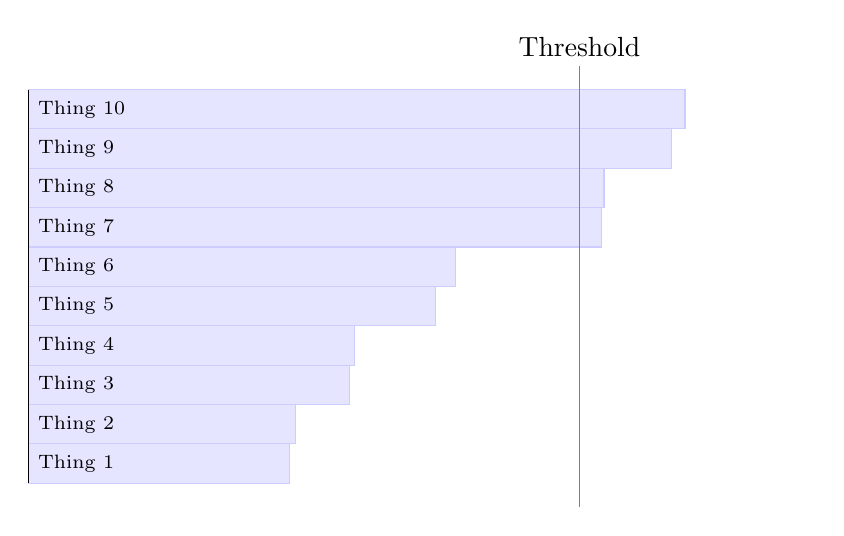
\begin{tikzpicture}[]
\begin{scope}[]
\clip (0,0) rectangle (10,5);
\begin{scope}[shift={(0.0,0.0)}]
\pgfsetxvec{\pgfpoint{0.028571429cm}{0cm}}
\pgfsetyvec{\pgfpoint{0cm}{0.5cm}}
\begin{scope}[draw=blue!20,fill=blue!10]
\pgfpathmoveto{ \pgfqpointxy {0.0} {10.0}}
\pgfpathlineto{ \pgfqpointxy {292.0} {10.0}}
\pgfpathlineto{ \pgfqpointxy {292.0} {9.0}}
\pgfpathlineto{ \pgfqpointxy {286.0} {9.0}}
\pgfpathlineto{ \pgfqpointxy {286.0} {8.0}}
\pgfpathlineto{ \pgfqpointxy {256.0} {8.0}}
\pgfpathlineto{ \pgfqpointxy {256.0} {7.0}}
\pgfpathlineto{ \pgfqpointxy {255.0} {7.0}}
\pgfpathlineto{ \pgfqpointxy {255.0} {6.0}}
\pgfpathlineto{ \pgfqpointxy {190.0} {6.0}}
\pgfpathlineto{ \pgfqpointxy {190.0} {5.0}}
\pgfpathlineto{ \pgfqpointxy {181.0} {5.0}}
\pgfpathlineto{ \pgfqpointxy {181.0} {4.0}}
\pgfpathlineto{ \pgfqpointxy {145.0} {4.0}}
\pgfpathlineto{ \pgfqpointxy {145.0} {3.0}}
\pgfpathlineto{ \pgfqpointxy {143.0} {3.0}}
\pgfpathlineto{ \pgfqpointxy {143.0} {2.0}}
\pgfpathlineto{ \pgfqpointxy {119.0} {2.0}}
\pgfpathlineto{ \pgfqpointxy {119.0} {1.0}}
\pgfpathlineto{ \pgfqpointxy {116.0} {1.0}}
\pgfpathlineto{ \pgfqpointxy {116.0} {0.0}}
\pgfpathlineto{ \pgfqpointxy {0.0} {0.0}}
\pgfusepath{ fill,stroke }
\end{scope}
\begin{scope}[draw=blue!20,fill=blue!10]
\pgfpathmoveto{ \pgfqpointxy {0.0} {10.0}}
\pgfpathlineto{ \pgfqpointxy {0.0} {10.0}}
\pgfusepath{ stroke }
\end{scope}
\begin{scope}[draw=blue!20,fill=blue!10]
\pgfpathmoveto{ \pgfqpointxy {0.0} {10.0}}
\pgfpathlineto{ \pgfqpointxy {292.0} {10.0}}
\pgfusepath{ stroke }
\end{scope}
\begin{scope}[draw=blue!20,fill=blue!10]
\pgfpathmoveto{ \pgfqpointxy {0.0} {9.0}}
\pgfpathlineto{ \pgfqpointxy {292.0} {9.0}}
\pgfusepath{ stroke }
\end{scope}
\begin{scope}[draw=blue!20,fill=blue!10]
\pgfpathmoveto{ \pgfqpointxy {0.0} {9.0}}
\pgfpathlineto{ \pgfqpointxy {286.0} {9.0}}
\pgfusepath{ stroke }
\end{scope}
\begin{scope}[draw=blue!20,fill=blue!10]
\pgfpathmoveto{ \pgfqpointxy {0.0} {8.0}}
\pgfpathlineto{ \pgfqpointxy {286.0} {8.0}}
\pgfusepath{ stroke }
\end{scope}
\begin{scope}[draw=blue!20,fill=blue!10]
\pgfpathmoveto{ \pgfqpointxy {0.0} {8.0}}
\pgfpathlineto{ \pgfqpointxy {256.0} {8.0}}
\pgfusepath{ stroke }
\end{scope}
\begin{scope}[draw=blue!20,fill=blue!10]
\pgfpathmoveto{ \pgfqpointxy {0.0} {7.0}}
\pgfpathlineto{ \pgfqpointxy {256.0} {7.0}}
\pgfusepath{ stroke }
\end{scope}
\begin{scope}[draw=blue!20,fill=blue!10]
\pgfpathmoveto{ \pgfqpointxy {0.0} {7.0}}
\pgfpathlineto{ \pgfqpointxy {255.0} {7.0}}
\pgfusepath{ stroke }
\end{scope}
\begin{scope}[draw=blue!20,fill=blue!10]
\pgfpathmoveto{ \pgfqpointxy {0.0} {6.0}}
\pgfpathlineto{ \pgfqpointxy {255.0} {6.0}}
\pgfusepath{ stroke }
\end{scope}
\begin{scope}[draw=blue!20,fill=blue!10]
\pgfpathmoveto{ \pgfqpointxy {0.0} {6.0}}
\pgfpathlineto{ \pgfqpointxy {190.0} {6.0}}
\pgfusepath{ stroke }
\end{scope}
\begin{scope}[draw=blue!20,fill=blue!10]
\pgfpathmoveto{ \pgfqpointxy {0.0} {5.0}}
\pgfpathlineto{ \pgfqpointxy {190.0} {5.0}}
\pgfusepath{ stroke }
\end{scope}
\begin{scope}[draw=blue!20,fill=blue!10]
\pgfpathmoveto{ \pgfqpointxy {0.0} {5.0}}
\pgfpathlineto{ \pgfqpointxy {181.0} {5.0}}
\pgfusepath{ stroke }
\end{scope}
\begin{scope}[draw=blue!20,fill=blue!10]
\pgfpathmoveto{ \pgfqpointxy {0.0} {4.0}}
\pgfpathlineto{ \pgfqpointxy {181.0} {4.0}}
\pgfusepath{ stroke }
\end{scope}
\begin{scope}[draw=blue!20,fill=blue!10]
\pgfpathmoveto{ \pgfqpointxy {0.0} {4.0}}
\pgfpathlineto{ \pgfqpointxy {145.0} {4.0}}
\pgfusepath{ stroke }
\end{scope}
\begin{scope}[draw=blue!20,fill=blue!10]
\pgfpathmoveto{ \pgfqpointxy {0.0} {3.0}}
\pgfpathlineto{ \pgfqpointxy {145.0} {3.0}}
\pgfusepath{ stroke }
\end{scope}
\begin{scope}[draw=blue!20,fill=blue!10]
\pgfpathmoveto{ \pgfqpointxy {0.0} {3.0}}
\pgfpathlineto{ \pgfqpointxy {143.0} {3.0}}
\pgfusepath{ stroke }
\end{scope}
\begin{scope}[draw=blue!20,fill=blue!10]
\pgfpathmoveto{ \pgfqpointxy {0.0} {2.0}}
\pgfpathlineto{ \pgfqpointxy {143.0} {2.0}}
\pgfusepath{ stroke }
\end{scope}
\begin{scope}[draw=blue!20,fill=blue!10]
\pgfpathmoveto{ \pgfqpointxy {0.0} {2.0}}
\pgfpathlineto{ \pgfqpointxy {119.0} {2.0}}
\pgfusepath{ stroke }
\end{scope}
\begin{scope}[draw=blue!20,fill=blue!10]
\pgfpathmoveto{ \pgfqpointxy {0.0} {1.0}}
\pgfpathlineto{ \pgfqpointxy {119.0} {1.0}}
\pgfusepath{ stroke }
\end{scope}
\begin{scope}[draw=blue!20,fill=blue!10]
\pgfpathmoveto{ \pgfqpointxy {0.0} {1.0}}
\pgfpathlineto{ \pgfqpointxy {116.0} {1.0}}
\pgfusepath{ stroke }
\end{scope}
\begin{scope}[draw=blue!20,fill=blue!10]
\pgfpathmoveto{ \pgfqpointxy {0.0} {0.0}}
\pgfpathlineto{ \pgfqpointxy {116.0} {0.0}}
\pgfusepath{ stroke }
\end{scope}
\begin{scope}[draw=blue!20,fill=blue!10]
\pgfpathmoveto{ \pgfqpointxy {0.0} {0.0}}
\pgfpathlineto{ \pgfqpointxy {0.0} {0.0}}
\pgfusepath{ stroke }
\end{scope}
\pgfsetxvec{\pgfpoint{1cm}{0cm}}
\pgfsetyvec{\pgfpoint{0cm}{1cm}}
\end{scope}
\end{scope}
\begin{scope}[xshift=0]
\draw[] [shift={(0.0,0.25)}] (0pt,0pt) -- (-0pt,-0pt) node[right]{ \scriptsize{Thing 1}};
\draw[] [shift={(0.0,0.75)}] (0pt,0pt) -- (-0pt,-0pt) node[right]{ \scriptsize{Thing 2}};
\draw[] [shift={(0.0,1.25)}] (0pt,0pt) -- (-0pt,-0pt) node[right]{ \scriptsize{Thing 3}};
\draw[] [shift={(0.0,1.75)}] (0pt,0pt) -- (-0pt,-0pt) node[right]{ \scriptsize{Thing 4}};
\draw[] [shift={(0.0,2.25)}] (0pt,0pt) -- (-0pt,-0pt) node[right]{ \scriptsize{Thing 5}};
\draw[] [shift={(0.0,2.75)}] (0pt,0pt) -- (-0pt,-0pt) node[right]{ \scriptsize{Thing 6}};
\draw[] [shift={(0.0,3.25)}] (0pt,0pt) -- (-0pt,-0pt) node[right]{ \scriptsize{Thing 7}};
\draw[] [shift={(0.0,3.75)}] (0pt,0pt) -- (-0pt,-0pt) node[right]{ \scriptsize{Thing 8}};
\draw[] [shift={(0.0,4.25)}] (0pt,0pt) -- (-0pt,-0pt) node[right]{ \scriptsize{Thing 9}};
\draw[] [shift={(0.0,4.75)}] (0pt,0pt) -- (-0pt,-0pt) node[right]{ \scriptsize{Thing 10}};
\end{scope}
\draw[thin,gray] (7.0,-0.3) -- (7.0,5.3);
\node at (7.0,5.3) [,above] {Threshold}; 
\begin{scope}[black]
\pgfpathmoveto{ \pgfqpointxy {0.0} {0.0}}
\pgfpathlineto{ \pgfqpointxy {0.0} {5.0}}
\pgfusepath{ stroke }
\end{scope}
\end{tikzpicture}
%%% Local Variables: 
%%% mode: latex 
%%% TeX-master: "master" 
%%% End:

